%!TEX root = ../report.tex
\chapter{Analysis}
\label{ch:analysis}

%All layers (with their patterns) is very clearly described in ch8 starting on p95.

Layering: 
\begin{itemize}
\item Service layer
\item Domain layer
\item Data source layer
\end{itemize}

\section{Layer Supertype}
\myworries{p475 POEAA
"A type that acts as the super type for all types in the layer".}

With this pattern, all the classes of a certain layer have the same super class. This super class then contains the features that are very common for the layer.

This pattern will be used in every layer.
\begin{description}
\item[Service layer] All the services need to take care of security. The client needs to be authenticated and the data needs to be decryption by the service layer. All this security logic will be placed in a super type using the "Layer Supertype" pattern In the service layer it contains the security logic.

\item[Domain layer]
\myworries{From book:
-  "Common features, such as the storage and handling of 'Identity Fields (216), can go there."}


\item[Data source layer]
The data mapper in the data source pattern can use a layer super type that handles all the common behavior, which can greatly reduce the extra work of coding. 

%(p308 (Metadata mapping pattern))
\end{description}

\section{Service layer}
The service layer exposes a set of services to be used by clients and for each service, there is a certain script that will be executed when the service is called. The service layer will be used with the "operation script" variation. This means that the Service Layer consists of thick classes that contain logic. 

\begin{quotation}
The easier question to answer is probably when not to use it. You probably don't need a Service Layer if your application's business logic will only have one kind of client - say, a user interface - and it's use case responses don't involve multiple transactional resources. [...]
But as soon as you envision a second kind of client, or a second transactional resource in use case responses, it pays to design in a Service Layer from the beginning.
\end{quotation}

\section{Domain layer}
The domain logic is complex and so it requires the use of the domain model pattern. This means that the domain is Object Oriented, with every class representing one specific, individual, meaningful part.
This is the most advanced pattern, reducing code duplication and increasing flexibility of the system.

The alternatives are : Transaction Script and Table module.

Transaction script: Each system call has its corresponding script that will be executed.\\
Table module: One class per table in the database that contains all the logic acting on that data.

\subsection{Unit of work}
\myworries{Do we need this? The domain might not be doing any analysis at all, it just uses spark for that.}

Provides concurrency control.

Analyzing the data can be computationally intensive, which is why multiple threads will be used do distribute the work. This requires coordination of the data that is being handled. The Unit of work pattern: ``Maintains a list of objects affected by a business transaction and coordinates the writing out of changes and the resolution of concurrency problems.''

\section{Data source layer}
The main database will be quite simple and the database actions won't be very complicated. However, the tables needed for the statistics can become very complex.

\begin{figure}[H]
\caption{Database structure draft}
\centering
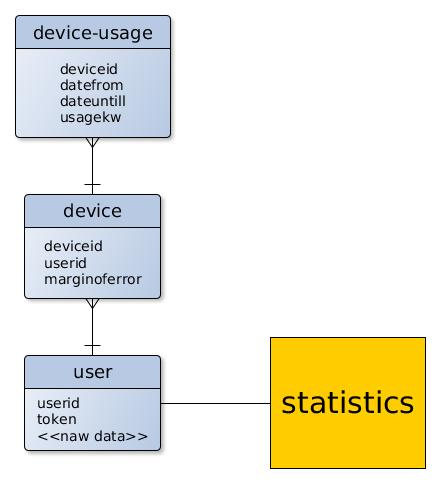
\includegraphics[]{4-analysis/images/SoftwarePatternsDatabaseDraft.jpg}
\end{figure}

Three main patterns to connect to data sources:

\begin{itemize}
\item Table data gateway (p144)
\item Row data gateway (p152)
\item Active record (p160)
\item Data mapper (p165)
\end{itemize}

Because the domain model is used in the domain layer, the data mapper pattern is best to use . (153 and 97)
The logic that will operate on the data will generate statistics of the data, which can become quite complex. This is why the data mapper pattern is chosen as a pattern for connecting to the data sources. This pattern is the most advanced pattern, but provides the best functionality and abstraction.

With the active record pattern, the database access/communication, data and logic of that data is all stored in the same class. Since the logic that will be executed on the sensor data is very complex, this patterns will not be useful.

A gateway of any kind leads to performance overhead, because for each call coming from the domain model pattern, a database call is made. It lacks the necessary coordination.

\subsection{Table data gateway}
\myworries{Not needed if the repository is used (i assume)}

The data mapper can use the table data gateway to remove the dependency on how the data is queried. Queries can be replaced with stored procedures in the Table data gateway without the data mappers having to change 

%Using a record set (504) turning into a unit of work (184)? P98 (lost the page:()

\subsection{Repository}
\myworries{
P322:
"Mediates between the domain and data mapping layers using a collection-like interface for accesing domain objects."
\\
P323:
"Repository supports the objective of achieving a clean separation and one-way dependency between the domain and data mapping layers"
\\
P324:
"Under the covers, Repository combines Metadata Mapping (329) with a Query object (316) to automatically generate SQL code from the criteria."
...
"In a large system with many domain object types and many possible queries, Repository reduces the amount of code needed to deal with all the querying that go's on."
}

The repository pattern mediates between the domain and data layer. The repository clients create a criteria object, specifying what kind of data is wanted. For example $criteria.equals(Person.LAST_NAME, Schaefers)$. Then the clients use this criteria by invoking repository.matching(criteria) to receive the data from the repository. The client just asks the data, it has no further knowledge about any interaction with any data source/data base.

The repository gives a lot more control over how the data is handled. The benefits are:
\begin{itemize}
\item Reduces code (and code complexity)
\item Increases performance
\item Separated domain and data layers, increasing flexibility and changeability
\end{itemize}

Performing analysis on the data also consists of executing complex queries on the data source. The database that executes these queries, however, might change. Or the system might decide to use multiple databases and data sources.
Using the Repository pattern, these changes can be made fast. The repository also allows for multiple configurations to exist. So an extra repository could be created for testing purposes, only using an in-memory database to increase the test execution speed.

\section{Client user interface}

\subsection{Controller}
\myworries{
On p 99:
\begin{itemize}
\item Given a free choice, I'd recommend Page Controller (p333). 
\item More complex navigation and UI lead you toward a Front Controller (344)
\end{itemize}
}
Page controller: controller for each page. So upon receiving a request do:
\begin{itemize}
\item decode url, extract data
\item invoke model to process data
\item determine view and use the model data to create the HTML to return
\end{itemize}

Front page controller:\\
One controller for all requests/views. This allows building a filter chain, handling authentication, logging etc.
Front page is better/helps with concurrency, because a new command object is created on each request. Reducing thread-safety concerns. \ign{(P346)}The model, however, can have shared objects that do require thread safety management.

The front page will be used, because it provides more functionality to the system. The only advantage of a page controller compared to the front controller is that it has a more natural structure.

\subsection{View}
\myworries{
Template view (350) or Transform view (361).
\\
(P forgot):
Template views have the edge at the moment.
}

Template view: Write HTML code including markers. Replace the markers with the data when the page is requested. (Play framework)\\
Transform view: convert the domain data to HTML, "transform" the domain data. Upon a request, it get the domain data, for each item in the data it looks for a appropriate "transform" to transform the data to HTML.

The template view will be used, because it is used a lot more then the transform view. Major web frameworks are based on this pattern (the play framework, laravel...). The view patterns don't have an important difference in how beneficial they are to the project.

%Transform view avoids having too much data in the HTML, because of the transform methods creating the HTML.
%Transform view can be tested without having a web server up.

\subsection{Model}
\myworries{
Communication with the model: p100:
Preference: Having everything run in one process if you can. Else Remote Facade (p388) and DTO (p 401).
}